\documentclass[10pt,xcolor={pst,svgnames},%,draft% ,handout
hyperref={
  pdfpagelabels=false,
  unicode=true,    
  pagebackref=true,
  hyperindex=true, 
  colorlinks=true, 
  breaklinks=true, 
  allcolors=black,
  bookmarks=true,  
  bookmarksopen=true,
}]{beamer}
\usepackage{bm}
\usepackage[beamer,en]{pop}
\usepackage{colortbl}
\usepackage{mathtools}
\usepackage{pgfpages}
%\setbeameroption{show notes on second screen=right}
\usepackage{xparse}
\usepackage{proof,mathpartir}
\usepackage{stmaryrd}
\usepackage{tikz}
\usepackage[all]{xy}
\usetikzlibrary{fit,calc,shapes,decorations.pathreplacing,positioning,automata,arrows,backgrounds,decorations.pathmorphing}
\tikzset{
  every overlay node/.style={
    % draw=black,fill=white,rounded corners,
    anchor=north west,
  },
}
\def\tikzoverlay{%
   \tikz[baseline,overlay]\node[every overlay node]
}%
\newcommand{\tikzmark}[1]{%
  \tikz[overlay,remember picture,yshift=.5ex]\node [inner sep=0] (#1) {};%
}

\newcommand{\DrawLine}[3][]{%
  \begin{tikzpicture}[overlay,remember picture]
    \draw[#1] (#2) -- (#3);
  \end{tikzpicture}
}
\tikzstyle{blop}=[circle,fill=black,inner sep=1]
\tikzstyle{token}=[circle,draw]
\tikzstyle{vert}=[thick,draw,circle,fill=blue!10,minimum height=15,inner sep=1]
\tikzstyle{bigvert}=[thick,draw,rounded corners=11pt,fill=blue!10,
minimum height=22,minimum width=22,inner sep=1]
\tikzstyle{state}=[thick,draw,circle,fill=blue!10,inner sep=1]
\tikzstyle{trans}=[thick,draw,minimum height=15,fill=yellow!30,inner sep=2]
\tikzstyle{transf}=[thick,draw,minimum height=15,fill=red!30,inner sep=2]
\tikzstyle{active}=[thick,draw,minimum height=15,fill=green!40]
\tikzstyle{blocked}=[thick,draw,minimum height=15,fill=red!40]
\tikzstyle{arc}=[thick,->,>=stealth]
\tikzstyle{every node}=[font=\footnotesize]
\tikzstyle{portnode}=[inner sep=0.2,outer sep=0.2]
\tikzstyle{portarc}=[->,>=latex]

\tikzstyle{every loop above}=[min distance=10mm,looseness=10]
\tikzstyle{uploop}=[out=55,in=125,loop, above]
\tikzstyle{dnloop}=[out=-125,in=-55,loop, below]
\tikzstyle{lfloop}=[out=145,in=-145,loop, left]
\tikzstyle{rgloop}=[out=-35,in=35,loop, right]
\tikzstyle{lbl}=[midway,fill=white,inner sep=1]

\DeclareDocumentCommand\initst{r()O{.8}}
{\draw[arc] ($ (#1) + (-#2,0) $) to (#1)}
\DeclareDocumentCommand\position{O{}O{above}r()r()}
{\node[state] (#3) at (#4) [label=#2:$#1$] {}}
\DeclareDocumentCommand\state{O{}r()r()}
{\node[state] (#2) at (#3) {$#1$}}
\DeclareDocumentCommand\transb{O{}r()r()}{
  \node[trans] (#2) at (#3) {};
  \node (l#2) at ($ (#3) + (0,0.6) $) {$#1$}}
\DeclareDocumentCommand\trans{O{}r()r()}
{\node[trans] (#2) at (#3) {$#1$}}
\DeclareDocumentCommand\transf{O{}r()r()}
{\node[transf] (#2) at (#3) {$#1$}}
\DeclareDocumentCommand\fnst{r()O{.8}}
{\draw[arc] (#1) to ($ (#1) + (#2,0) $)}
\DeclareDocumentCommand\edge{O{above}O{midway}r()r()O{}}
{\draw[arc] (#3) to[#1] node[#2]{$#5$} (#4)}
\DeclareDocumentCommand\cedge{O{red} O{above}O{midway}r()r()O{}}
{\draw[arc,#1] (#4) to[#2] node[#3]{$#6$} (#5)}
% \DeclareDocumentCommand\token[2]{\filldraw[fill=#2] (#1) circle [radius=0.05]}
\DeclareDocumentCommand\etat{O{}r()r()}
{\node[state,minimum height=4ex]
  (#2) at (#3) {$#1$}}
\DeclareDocumentCommand\final{O{1,0}r()}{
  % \draw[thick,dotted,fill=red!10] ($ (#1) + (-0.4,-0.4) $) rectangle ($ (#1) + (0.4,0.4) $)
  \transf (fntr) ($(#2)+(#1)$);
  \edge(#2)(fntr);
}

\DeclareDocumentCommand\auto{O{0,0}r()r()}{
  \draw[>=latex,out=40,in=140,fill=gray!10] (#3)
  to ($ (#3) + (1.5,0) + (#1) + (#1)$) to [in=-40,out=-140]  (#3);
  \etat[\iota_#2] (i#2) (#3);
  \etat[f_#2] (f#2) ($ (i#2) + (1.5,0) + (#1) + (#1)$);
  \node (lbl#2) at ($ (i#2) + (0.75,0) + (#1)$) {$e_{#2}$}% ;
  % \draw[thick,>=latex,out=30,in=150] (i#2) to (f#2);
  % \draw[thick,>=latex,out=-30,in=-150] (i#2) to (f#2)
}

\DeclareDocumentCommand\clbox{ O{.25} r() O{.25} r() }{
  \draw  ($(#2)-(.25,#1)$) rectangle ($(#4)+(.25,#3)$)
}

\DeclareDocumentCommand\rect{ O{.5} r() r() O{.5} r() r()}{
  \draw  ($(#2-|#3)-(.25,#1)$) rectangle ($(#5-|#6)+(.25,#4)$)
}

\newcommand\port[4]{   
  \node[portnode] (#3) at ($(#4)+(#1)$){$#2$};
  \draw[portarc]  (#3) to (#4)
}
\DeclareDocumentCommand\iport{ O{0} r() o r() o }
{
  \IfNoValueTF{#5}{
    \IfNoValueTF{#3}
    {\port{-.6,#1}{#2}{p#2i}{#4}}
    {\port{-.6,#1}{#2}{#3}{#4}}
  }{
    \IfNoValueTF{#3}
    {\node[portnode] (p#2i) at ($(#5|-#4)+(-.6,#1)$){$#2$};
      \draw[portarc]  (p#2i) to (#4)
    }
    {\node[portnode] (#3) at ($(#5|-#4)+(-.6,#1)$){$#2$};
      \draw[portarc]  (#3) to (#4)
    }
    
  }
}
\DeclareDocumentCommand\oport{ O{0} r() o r() o }
{
  \IfNoValueTF{#5}{
    \IfNoValueTF{#3}
    {\port{.6,#1}{#2}{p#2o}{#4}}
    {\port{.6,#1}{#2}{#3}{#4}}}{
    \IfNoValueTF{#3}
    {\node[portnode] (p#2o) at ($(#5|-#4)+(.6,#1)$){$#2$};
      \draw[portarc]  (p#2o) to (#4)
    }
    {\node[portnode] (#3) at ($(#5|-#4)+(.6,#1)$){$#2$};
      \draw[portarc]  (#3) to (#4)
    }
    
  }
}
% \DeclareDocumentCommand\hdist{ r() r() }{
%   ($(#1|-#2)!.5!(#2)-(#1|-#2)$)
% }
% \DeclareDocumentCommand\vdist{ r() r() }{
%   ($(#1|-#2)!.5!(#2)-(#2)$)
% }
\newcommand\hdist[2]{
  ($(#2)-(#1|-#2)$)
}
\newcommand\vdist[2]{
  ($(#1)-(#1|-#2)$)
}

%%% Local Variables:
%%% mode: latex
%%% TeX-master: "../main"
%%% End:

\usepackage{listings}
\usepackage{fmtcount}
\usepackage{colortbl}
%\usepackage{hyperref}
%\usepackage{fancybox}
\hypersetup{
  pdftitle={Algebras of Relations},
  pdfauthor={Paul Brunet},
  pdfsubject={Kleene Algebra}}
%\addtobeamertemplate{footline}{\hypersetup{allcolors=.}}{}


\NewDocumentCommand\DownArrow{O{2.0ex} O{black} O{}}{%
   \mathrel{\tikz[baseline] \draw [<-, line width=0.5pt, #2] (0,0) -- ++(0,#1) node[midway, right] {#3};}
}

\newcolumntype{M}[1]{>{\centering\arraybackslash}m{#1}}

\newcommand\mailto[1]{\href{mailto:#1}{\nolinkurl{#1}}}

\newcommand\simplecite[3]{
  {\color{basecolor!80!black}%
    \footnotesize {#1}, {\small{\bf #2}}, {\footnotesize\textit{#3}}}
} 

\definecolor{celadon}{rgb}{0.67, 0.88, 0.69}
\definecolor{bubblegum}{rgb}{0.99, 0.76, 0.8}

\beamerboxesdeclarecolorscheme{vert}{celadon!70}{celadon!50}
\beamerboxesdeclarecolorscheme{rose}{bubblegum!70}{bubblegum!50}
%\beamerboxesdeclarecolorscheme{gris}{gris!10}{gris!10}
%\beamerboxesdeclarecolorscheme{bleu}{cyan!10}{cyan!10}
%\beamerboxesdeclarecolorscheme{rosebis}{rose!60}{rose!15}
%\beamerboxesdeclarecolorscheme{vertbis}{vert!60}{vert!15}
%\beamerboxesdeclarecolorscheme{rouge}{red!10}{red!30}
%\beamerboxesdeclarecolorscheme{jaune}{yellow!10}{yellow!10}
%\beamerboxesdeclarecolorscheme{vert}{vert!10}{vert!30}
%\beamerboxesdeclarecolorscheme{vertp}{vert!10}{vert!10}

\newcommand\set[1]{\left\{#1\right\}}
\newcommand\tuple[1]{\langle{#1}\rangle}
\newcommand\paren[1]{\left({#1}\right)}
\newcommand\pset[1]{\mathcal P\paren{#1}}
\newcommand\setcompr[2]{\set{#1\ \left|\ #2\right.}}
\newcommand\Mid{\mathrel{~\mid~}}

% divers
\newcommand\eqdef\coloneqq
\renewcommand\hat\widehat

% perso
\renewcommand\G{\mathpzc G}
\renewcommand\C{\mathpzc C}
\newcommand\T{\mathpzc T}
\newcommand\F{\mathpzc F}
\newcommand\B{\mathcal B}
\renewcommand\L{\mathpzc L}

\newcommand\KLm{$\text{KL}$}
\newcommand\KA{$\text{KA}$}

\newcommand\Un{% \mathbb
  1}
\newcommand\Zero{% \mathbb
  0}
\newcommand\pspace{% \textsc
  {PSpace}}
\newcommand\expspace{% \textsc
  {ExpSpace}}
\newcommand\converse{\smallsmile}
\newcommand\conv[1]{{#1}^\converse}

\newcommand\id[1]{\text{Id}_{#1}}
\newcommand\reg[1][\Sigma]{\text{Reg}\tuple{#1}}
\newcommand\sqreg[1][\Sigma]{\text{Reg}^2\tuple{#1}}
\newcommand\areg[1][\Sigma]{\text{AReg}\tuple{#1}}
\newcommand\imreg[1][\Sigma]{\text{IMReg}\tuple{#1}}
\newcommand\imregm[1][\Sigma]{\text{IMReg}^-\tuple{#1}}
\newcommand\cireg[1][\Sigma]{\text{Reg}^{\converse\cap}\tuple{#1}}
\newcommand\creg[1][\Sigma]{\text{Reg}^{\converse}\tuple{#1}}
\newcommand\ireg[1][\Sigma]{\text{GReg}\tuple{#1}}
\newcommand\regm[1][\Sigma]{\text{Reg}^-\tuple{#1}}
\newcommand\tm[1][\Sigma]{\mathbb{W}_{#1}}
\newcommand\iregf[1][\Sigma]{\text{Reg}^{\cap}\tuple{#1}}
\newcommand\GT[1][\Sigma]{\text{W}_{#1}}
\newcommand\GTm[1][\Sigma]{\GT[#1]^-}
\newcommand\argument\_

\newcommand\lang[1]{\L\paren {#1}}
\newcommand\Rel{\mathrm{Rel}}
\newcommand\Lang{\mathrm{Lang}}
\newcommand\ka{\mathrm{KA}}
\newcommand\cka{\mathrm{KAC}}

\newcommand\ok{{\color{green}\fontencoding{U}\fontfamily{ding}%
\selectfont\symbol{'041}}}
\newcommand\nope{{\color{red}\fontencoding{U}\fontfamily{ding}%
\selectfont\symbol{'045}}}
\newcommand\quest{
  \scalebox{1.5}{{\color{orange}\usefont{OT1}{pbk}{m}{n} ?}}
}
\definecolor{lightgray}{gray}{.7}
\newcommand\okg{{\color{lightgray}\fontencoding{U}\fontfamily{ding}%
\selectfont\symbol{'041}}}
\newcommand\nopeg{{\color{lightgray}\fontencoding{U}\fontfamily{ding}%
\selectfont\symbol{'045}}}
\newcommand\questg{
  \scalebox{1.5}{{\color{lightgray}\usefont{OT1}{pbk}{m}{n} ?}}
}

\newcommand\dom[1]{\text{dom}\paren{#1}}
\newcommand\img[1]{\text{img}\paren{#1}}
\newcommand\Tr[1]{\G\paren{#1}}
\newcommand\Pm[1]{\lang{#1}}
\newcommand\Ln[1]{\L\paren{#1}}

\newcommand\duck\preccurlyeq
\newcommand\lessgr\blacktriangleleft
\newcommand\gtgr\blacktriangleright

\newcommand\sigdot{{\Sigma'}}

\newcommand\clgt[1]{\prescript{\lhd}{}{#1}} 
\newcommand\clgr[1]{\prescript{\lessgr}{}{#1}}
\newcommand\qmequiv{\mathrel{%
    \mathchoice{\QMEQUIV}{\QMEQUIV}{\QMEQUIV}{\QMEQUIV}%
}}
\newcommand\QMEQUIV{{%
    \setbox0\hbox{$\xLeftrightarrow{\quad}$}%
    \rlap{\hbox to \wd0{\hss?\hss}}\box0
}}
\newcommand\nmodels{\mathrel{%
    \mathchoice{\NMODELS}{\NMODELS}{\NMODELS}{\NMODELS}%
}}
\newcommand\NMODELS{{%
    \setbox0\hbox{$\models$}%
    \rlap{\hbox to \wd0{\hss\textbf{\small\color{red}/}\hss}}\box0
}}
\newcommand\redneq{\mathrel{%
    \mathchoice{\REDNEQ}{\REDNEQ}{\REDNEQ}{\REDNEQ}%
}}
\newcommand\REDNEQ{%
    \setbox0\hbox{$=$}%
    \rlap{\hbox to \wd0{\hss\textbf{\small\color{red}/}\hss}}\box0
}
\newcommand\modelplop{\mathrel{%
    \mathchoice{\MODEL}{\MODEL}{\MODEL}{\MODEL}%
}}
\newcommand\MODEL{{%
    \setbox0\hbox{$\models$}%
    \rlap{\hbox to \wd0{\hss\textbf{\small\color{red}}\hss}}\box0
}}

\newtheorem{cntrexample}{Counterexample}
\newenvironment<>{cntrexample}[1][]{%
  \setbeamercolor{block title}{fg=white,bg=green!75!blue}%
  \begin{block}#2{Counterexample\def\temp{#1}\ifx\temp\empty\else ~(#1)\fi}}{\end{block}}

\renewenvironment{proof}{\emph{Proof.}}{\hfill\emph{$\Box$}}
\renewcommand\emph[1]{{\color{basecolor!80!black}\textbf{#1}}}
%% Title page...

\newcommand{\inclhom}{\stackrel{\blacktriangleleft}{\subseteq}}
\newcommand\I{\mathcal I}
\renewcommand\K{\mathcal K}
\renewcommand\A{\mathcal A}
\renewcommand\L{\mathcal L}
\newcommand\V{\mathcal V}
\newcommand\fresh{\mathrel{\#}}
\newcommand\perm[1]{\paren{#1}}
\newcommand\eperm[1]{\left\langle{#1}\right\rangle}
\newcommand\prove[3][Ax]{#1\vdash #2 = #3}
\newcommand\iprove[3][Ax]{#1\vdash #2 \leqslant #3}
\newcommand\fpset[1]{\mathcal P_f\paren{#1}}



\newcommand{\expr}{\mathbb E}
\newcommand{\typed}{\mathbb T}
\newcommand{\untyped}{\mathbb U}
\newcommand{\single}{\expr\tuple{\A}}
\newcommand{\multi}{\expr\tuple{X}}
\newcommand{\singlep}{\expr^+\tuple{\A}}
\newcommand{\multip}{\expr^+\tuple{X}}
\newcommand{\positive}{\mathbb E^+}
\newcommand{\noperm}{\mathbb C}
\newcommand{\trees}{\mathcal{T}}

\xdefinecolor{darkgreen}{named}{DarkGreen}
\xdefinecolor{dimgray}{named}{DimGray}
\xdefinecolor{brown}{named}{Brown}


\setbeamertemplate{itemize items}[default]
\setbeamertemplate{enumerate items}[default]
\setbeamertemplate{headline}{%
\leavevmode%
  \hbox{%
  \begin{beamercolorbox}[wd=.5\paperwidth,ht=2.5ex,dp=1.125ex]{section in head/foot}%
    \hfill\usebeamerfont{section in head/foot}\insertsectionhead\hspace{.5cm}
  \end{beamercolorbox}%
  \begin{beamercolorbox}[wd=.5\paperwidth,ht=2.5ex,dp=1.125ex]{subsection in head/foot}%
    \hspace{.5cm}\usebeamerfont{subsection in head/foot}\insertsubsectionhead
  \end{beamercolorbox}}%% %
  %   \begin{beamercolorbox}[wd=\paperwidth,ht=2.5ex,dp=1.125ex]{palette primary}%
  %     \insertsubsectionnavigationhorizontal{\paperwidth}{}{}
  %   %\insertsectionnavigationhorizontal{\paperwidth}{}{}
  %   \end{beamercolorbox}%
  % }
}
\renewcommand\thesection{\Roman{section}}
\setbeamertemplate{section in toc}{
  \MakeUppercase{\romannumeral\inserttocsectionnumber.}~\inserttocsection}

\setbeamertemplate{subsection in toc}{%
  \hspace{1.2em}{\color{basecolor!80!black}\scriptsize\raise1.25pt
    \hbox{\donotcoloroutermaths$\blacktriangleright$}}%
  ~\inserttocsubsection\par}
\graphicspath{{img/}}
\renewenvironment{proof}{\emph{Proof.}}{\hfill\emph{$\Box$}}


\title[Relation Algebra]
{Regular and first-order tree-to-tree functions}
%
\author{\underline{Amina Doumane} \& Mikołaj Bojańczyk}
%% Headers for other pages...

\institute{LIP-ENS Lyon}

\subtitle{}

\subject{Algèbre de Kleene}
\titlegraphic{%
  \begin{minipage}{1\linewidth}
    \centering
   
\includegraphics[width=.20\textwidth]{logos/LIP.png}
  \end{minipage}
%
% \hfill\includegraphics[width=.15\textwidth]{logos/logo_lip.png}%
% \hfill\includegraphics[width=.15\textwidth]{logos/logo_lyon1.png}%
% \hfill\includegraphics[width=.15\textwidth]{logos/logo_univlyon.png}%
%\hfill%
}

\date{September \ordinalnum{18}, 2019}
\addtobeamertemplate{footline}{\hypersetup{allcolors=.}}{}
\addtobeamertemplate{headline}{\hypersetup{allcolors=.}}{}
\begin{document}
\tikzset{every state/.style={thick,draw,circle,inner sep=1,minimum size=2ex}}\tikzset{every picture/.style={thick}}
%\tikzset{thick}
\tikzset{node distance=2cm}
\tikzset{>=stealth}
\tikzset{initial text={}}


\begin{frame}[plain]
  \bibliographystyle{apalike}
  %\bibliographystyle{abbrvurl}
  \nobibliography{short,mybibli}
  \titlepage 
\note{This is a joint work with Mikolaj Bojanczyk.}
 \end{frame}
%\part{Algebras of Binary Relations}
%\section{Introduction}

\begin{frame}
\frametitle{Regular and first-order word transductions}
$${f: A^* \to B^*}$$
\vfill
\begin{center}
$\begin{array}{>{\centering\arraybackslash}m{.3\textwidth} >{\centering\arraybackslash}m{.31\textwidth}>{\centering\arraybackslash}m{.32\textwidth}}
\hline
\cellcolor{celadon!50} Streaming string transducers (SST) &    
\begin{tikzpicture}[scale=.7, initial text = {}]
    \tikzstyle{every node}=[font=\scriptsize]
    \node[state,initial] (1) at (-.5,0) {$q_0$};
    \node[state, accepting] (2) at (3,0){$q_1$};
     \path (2) edge[uploop] node[above]{\scalebox{1}{$\begin{array}{l|l}
  a& R:=S $\quad$\\ &S:=bR$\quad$
   \end{array}$}
   } (2);
   \edge (1) (2)[\scalebox{1}{$\begin{array}{l|l}
  b& R:=aR $\quad$\\ &S:=bS$\quad$
   \end{array}$}];\end{tikzpicture}
     & \cellcolor{bubblegum!50} Monotone SST
\rule[-1cm]{0pt}{2cm} \\\hline\cellcolor{celadon!50}  MSO transductions & $x\geq y \mapsto y\geq x$ & \cellcolor{bubblegum!50}  FO transductions \rule[-1cm]{0pt}{2cm} \\\hline
\cellcolor{celadon!50}  List functions &  $\ \ $ Basic functions $\qquad$ (eg. $ abaa \mapsto aaba$) $\qquad$ + compositon & \cellcolor{bubblegum!50}  FO list functions  \rule[-1cm]{0pt}{2cm} \\\hline
\end{array}$
\end{center}
\vfill
\note{Our starting point was the nice equivalent caraterizations of regular string to string functions. Here you can see three formalisims defining the same class of function. The first one is based on transducers, the second one, MSO transductions, sees a word as a structure and uses formulas to describe the link between the input and the output. The last one uses some prime functions for instance the reverse function, which can be combined by composition to obtain all regular functions. And we have the same picture for first order transductions by adding some restrictions in the threee formalisms.  }
\end{frame}

\begin{frame}
\frametitle{Regular and first-order tree-to-tree transductions}
$${f: \trees(A) \to \trees(B)}$$
\vfill
\begin{center}
$\begin{array}{>{\centering\arraybackslash}m{.45\textwidth}} 
\hline
\cellcolor{celadon!50} Streaming tree transducers (STT) 
\rule[-1cm]{0pt}{2cm} \\\hline\cellcolor{celadon!50}  MSO transductions \rule[-1cm]{0pt}{2cm} \\\hline
\cellcolor{celadon!50}  \only<1>{?}\only<2>{\textbf{Tree-to-tree functions}}   \rule[-1cm]{0pt}{2cm} \\\hline
\end{array}$
\hfill
$\begin{array}{>{\centering\arraybackslash}m{.45\textwidth}}
\hline \cellcolor{bubblegum!50} Monotone STT
\rule[-1cm]{0pt}{2cm} \\\hline
 \cellcolor{bubblegum!50}  FO transductions \rule[-1cm]{0pt}{2cm} \\\hline \cellcolor{bubblegum!50}  \only<1>{?}\only<2>{\textbf{FO tree-to-tree functions}}  \rule[-1cm]{0pt}{2cm} \\\hline
\end{array}$

\end{center}
\note{Now, if we move to tree-to-tree functions, the situation is promising: we have a trasducer formualism, which is equivalent to MSO transductions. The goal of this work is to generalise to trees the approach using building blocks. And by that I mean finding a a reasonnable set of functions which genreates the regular transductions by composition.}
\end{frame}

\begin{frame}\frametitle{Regular and first-order tree-to-tree functions}
$${f: \trees(A) \to \trees(B)}$$\vspace{-1cm}
$$
\begin{array}{>{\centering\arraybackslash}m{.5\textwidth}>{\centering\arraybackslash}m{.5\textwidth}}
\scalebox{.8}{$\mathsf{unit}: A\to \trees(A)$} & \scalebox{.8}{$\mathsf{flat}: \trees(\trees(A)) \to \trees(A) $} \rule[-1cm]{0pt}{2cm} \\[-.5cm]
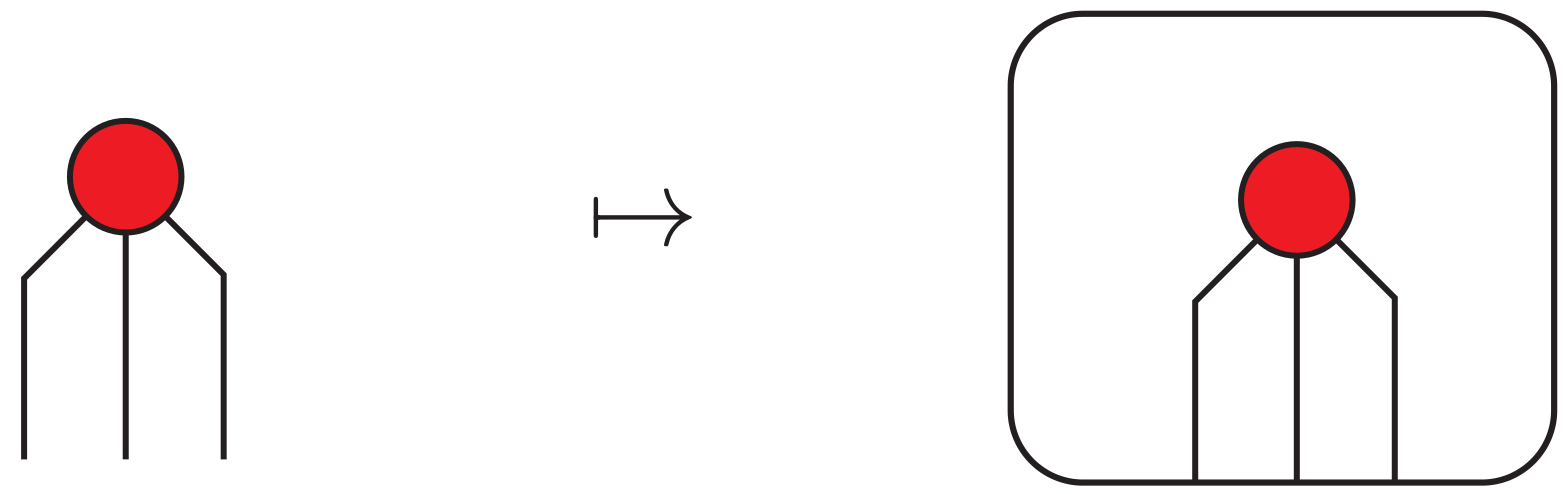
\includegraphics[scale=.07]{unit.png} & 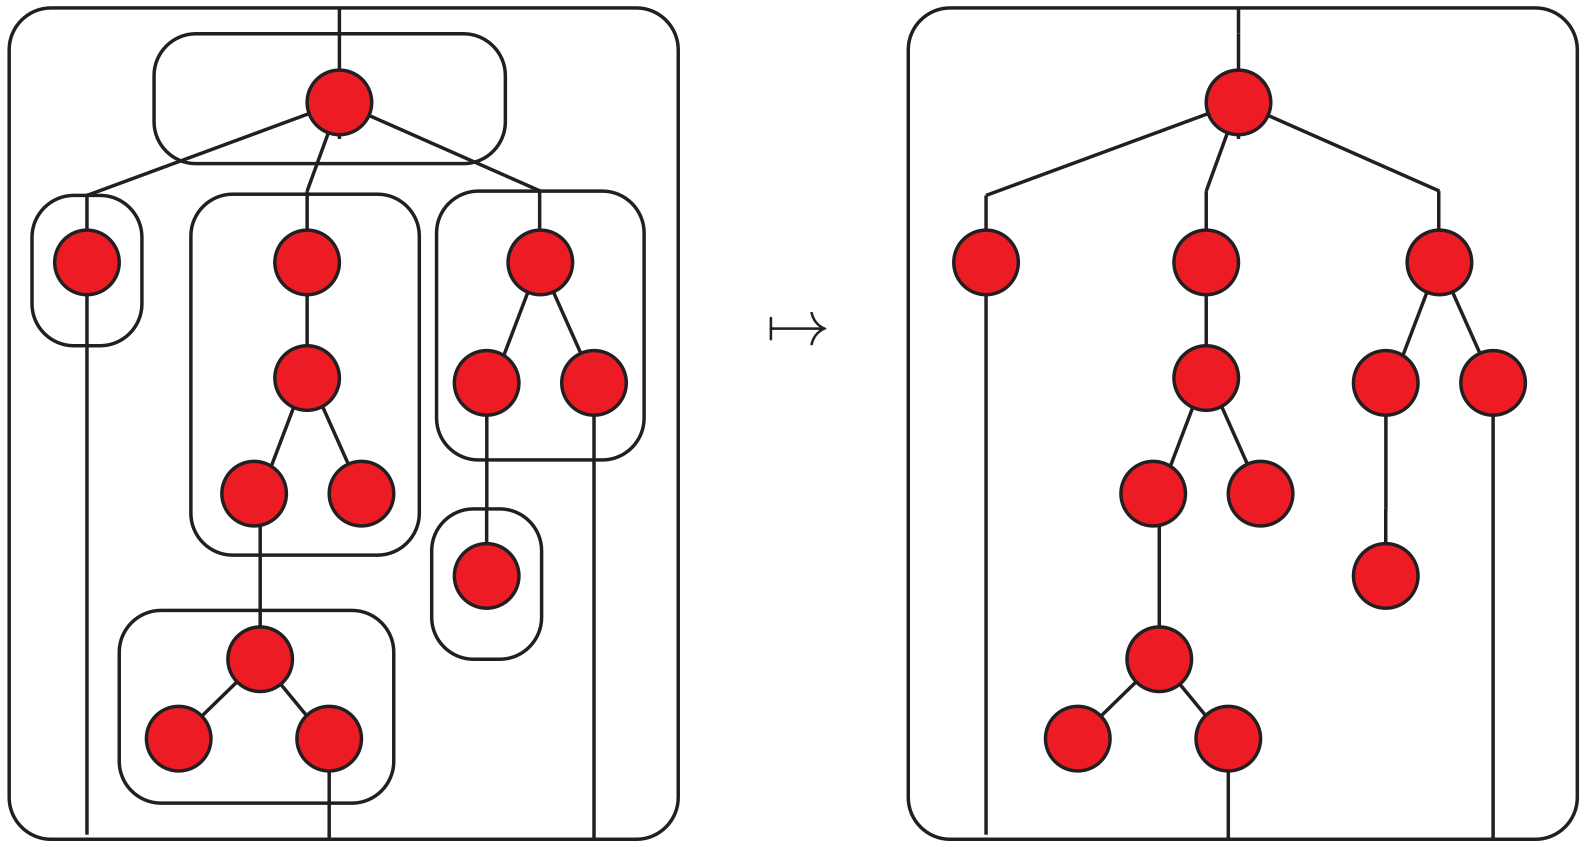
\includegraphics[scale=.07]{flat.png}  \\[-.5cm]
\scalebox{.8}{$\text{Depth-first-search}:\trees(A) \to \trees(A)$} &  \scalebox{.8}{$\mathsf{block}: \trees(A+B) \to \trees(\trees(A)+\trees(B))$} \rule[-1cm]{0pt}{2cm} \\[-.5cm]
\vspace{-.5cm}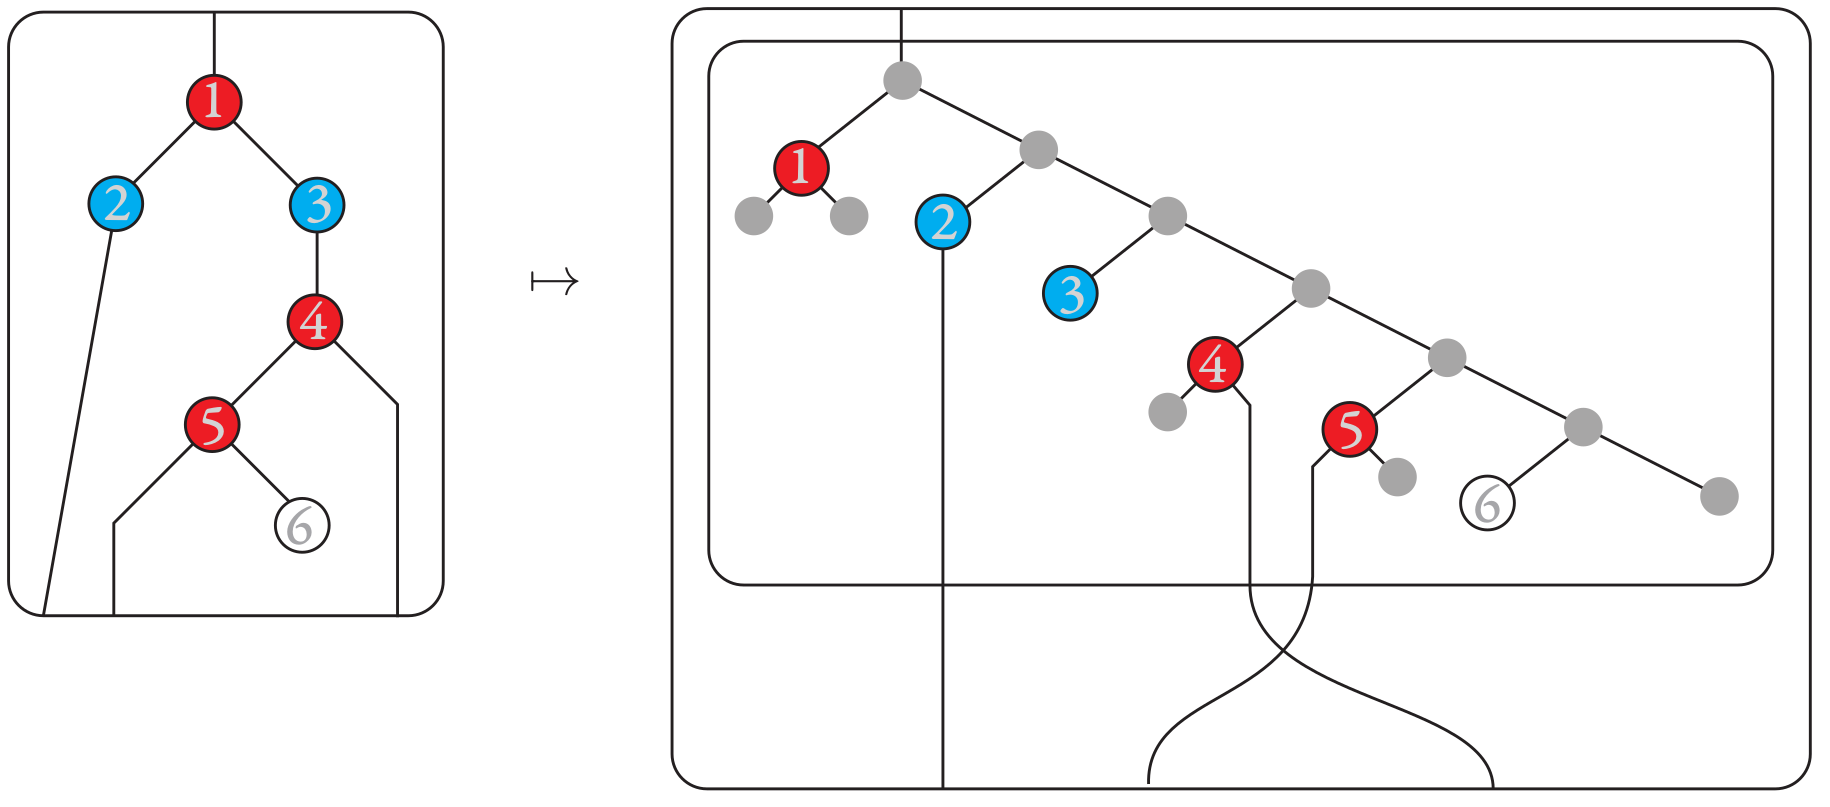
\includegraphics[scale=.07]{preorder.png} & 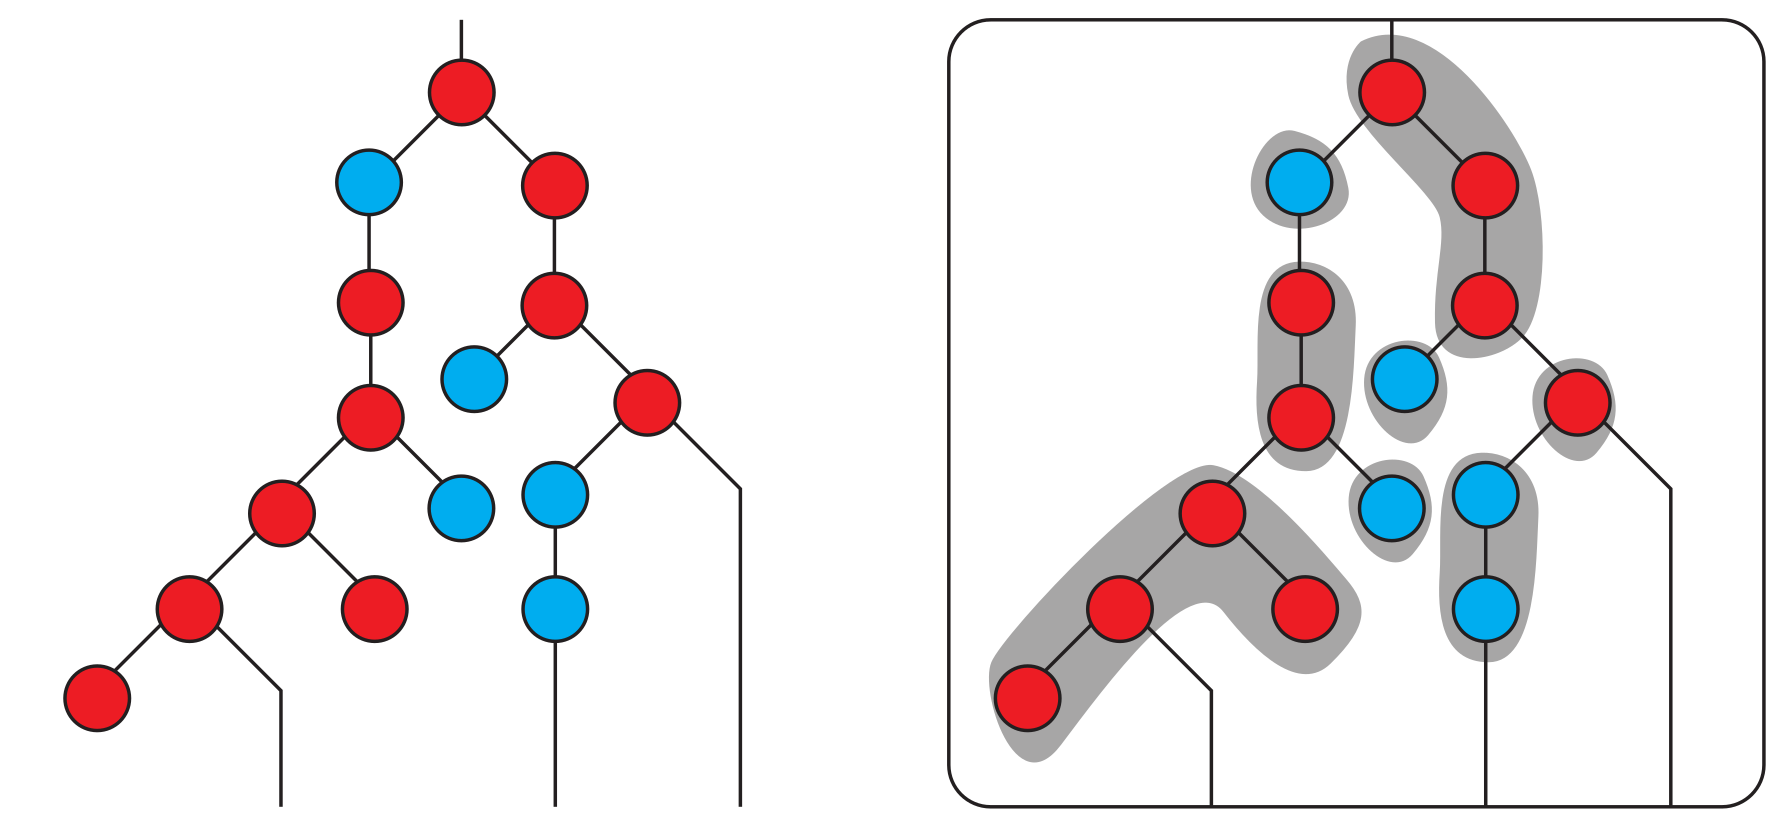
\includegraphics[scale=.07]{block.png} \ \  \rule[-1cm]{0pt}{2cm} 
\end{array}
$$
\note{Here are some examples of our basic functions.

Our alphabets are ranked, which means that every letter has an arity. 

In order to have an elegant and simple set of functions, our building blocks can have complex types, typically they can be functions from letters to trees like the function unit, or from trees of trees to trees, like the function flat.
Another examples of basic function is the depth-first search function, whilch builds a comb describing the depth first search visiting order. Finally, we have the block function, which groups together letters from the same subalphabet.
}
\end{frame}

\begin{frame}\frametitle{Regular and first-order tree-to-tree functions}
\hspace{-.3cm} 
\begin{tabular}{cc}
\begin{minipage}{.47\linewidth}
 \begin{beamerboxesrounded}[scheme=vert]{\textcolor{blue}{Theorem}} 
Term functions = MSO transductions\hspace{-.4cm} 
\end{beamerboxesrounded}
\end{minipage}
&
\begin{minipage}{.48\linewidth}
\begin{beamerboxesrounded}[scheme=rose]{\textcolor{blue}{Theorem}} 
FO term functions = FO transductions
\end{beamerboxesrounded}
\end{minipage}
\end{tabular}
\vfill
\begin{tabular}{cc}
\begin{minipage}{.47\linewidth}
 \begin{block}{By product 2}
Temporal logic for trees corresponding to FO.
\end{block}
\end{minipage}
&
\begin{minipage}{.48\linewidth}
 \begin{block} {By product 2}
Evaluation of simply typed linear $\lambda$-terms is a FO transduction.
\end{block}
\end{minipage}
\end{tabular}
\end{frame}


\begin{frame}\frametitle{What's next?}
\begin{itemize}
\item Implementations \vfill
\item Graph-to-graph functions \vfill
\item Poly-regular functions \vfill
\end{itemize}
\pause
\begin{center}
\vfill 
\textbf{Thank you for your attention!}
\end{center}
\end{frame}
\end{document}


\begin{frame}\frametitle{(First-order) Term functions: Completeness}
\hspace{-.3cm} 
\begin{tabular}{cc}
\begin{minipage}{.47\linewidth}
 \begin{beamerboxesrounded}[scheme=vert]{\textcolor{blue}{Theorem}}
STT functions $\subseteq$ Term functions
\end{beamerboxesrounded}
\end{minipage}
&
\begin{minipage}{.48\linewidth}
 \begin{beamerboxesrounded}[scheme=rose]{\textcolor{blue}{Theorem}} 
Monotone STT  $\subseteq$ FO term functions
\end{beamerboxesrounded}
\end{minipage}
\end{tabular}
\vfill
\onslide<2->{
\begin{center}
\begin{tikzpicture}[scale=.7, initial text = {}]
    \tikzstyle{every node}=[font=\scriptsize]
    \node (1) at (0,0) {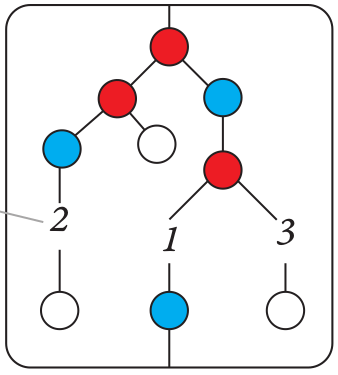
\includegraphics[scale=.2]{lambda1.png}};
    \onslide<3->{\node (2) at (6,0){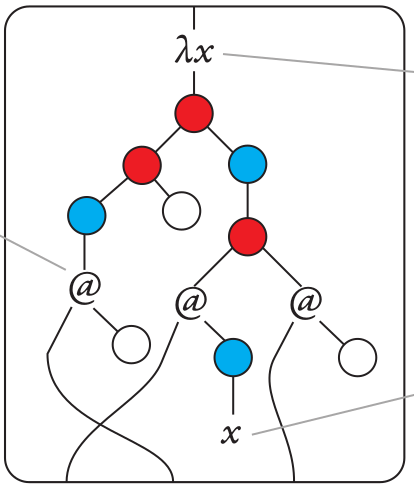
\includegraphics[scale=.2]{lambda2.png}};}
    \node (3)at (12,0){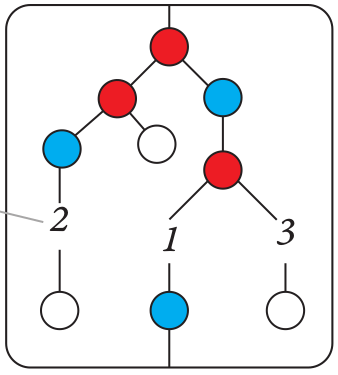
\includegraphics[scale=.2]{lambda3.png}};
    \only<2>{ \edge (1) (3)[\text{Computation of an STT}];}
  \onslide<3->{ \edge (1) (2)[\text{Relabeling}];
   \edge (2) (3)[\beta\text{-reduction}];}
   \end{tikzpicture}
\end{center} }
\onslide<4->{
\hspace{-.3cm} 
\vfill
}
\end{frame}

\begin{frame}
\frametitle{Regular and star-free word languages}
$${L: A^* \to \{\text{yes, no}\}}$$
\vfill
\begin{center}
$\begin{array}{>{\centering\arraybackslash}m{.3\textwidth} >{\centering\arraybackslash}m{.3\textwidth}>{\centering\arraybackslash}m{.32\textwidth}}
\hline
\cellcolor{celadon!50} NFA&    
\begin{tikzpicture}[scale=.7, initial text = {}]
    \tikzstyle{every node}=[font=\scriptsize]
    \node[state,initial] (1) at (0,0) {$q_0$};
    \node[state] (2) at (1.5,0){$q_1$};
    \node[state, accepting] (3)at (3,0){$q_2$};
     \path (2) edge[uploop] node[above]{a,b
   } (2);
   \edge (1) (2)[a];\edge (2) (3)[b];\end{tikzpicture}

     & \cellcolor{bubblegum!50} Counter-free NFA
\rule[-1cm]{0pt}{2cm} \\\hline\cellcolor{celadon!50}  MSO over words & {$\forall x. a(x) \vee b(\mathsf{succ}(y))$} & \cellcolor{bubblegum!50}  FO over words \rule[-1cm]{0pt}{2cm} \\\hline
\cellcolor{celadon!50}  Regular expressions &  $a\cdot((b+a)^*\cdot b)^c$ & \cellcolor{bubblegum!50}  $\star$-free regular expressions \rule[-1cm]{0pt}{2cm} \\\hline
\end{array}$
\end{center}
\vfill
%\textbf{Many other characterizations: monoids, grammars, temporal logics$\dots$}
\note{Parmis les raison qui font que }
\end{frame}
